% Template build by Guus Klinkenberg 
% He can be reached by email: 
% ineedanemailforlicensestuff@gmail.com

% This template is licensed under a Attribution-NonCommercial-ShareAlike Creative Commons 3.0 license
% http://creativecommons.org/licenses/by-nc-sa/3.0/

% The effects of this license are that you can you use it, and alter it, as long as you redistribute it.
% Keep in mind this is a non-commercial license.
% YOU ARE NOT ALLOWED TO USE IT FOR COMMERCIAL PURPOSES, unless allowed by the author of the template.

% The original author would love to keep this line and everything above it the same, but he cannot force you to.

% Document class.
\documentclass{article}

% Hyphonation for text and url
\usepackage[english]{babel}
\usepackage[hyphens]{url}

%Enable bibliography
\usepackage[numbers]{natbib}

% Accept é ë etc
\usepackage[utf8]{inputenc}
\usepackage[T1]{fontenc}
% Thanks, Laura Baakman

% More fonts and symbols
\usepackage{textcomp}
\usepackage{amsfonts}

% Allow for more symbols etc
\usepackage{verbatim}
\usepackage{marvosym}
\usepackage{amsmath}

% Math... and stuff
\usepackage{mathtools}

% Colors etc
\usepackage{color}
\usepackage[usenames,dvipsnames]{xcolor}
\definecolor{light-gray}{gray}{0.95}

% Listings and other mark up
\usepackage{listings}
\usepackage{verbatim}
\usepackage{appendix}
\usepackage{hyperref}

% Define the style of lstlisting
\lstset{ %
language=java,        						% choose the language of the code
basicstyle=\ttfamily,       				% the size of the fonts that are used for the code
numbers=left,        	          			% where to put the line-numbers
numberstyle=\footnotesize,			      	% the size of the fonts that are used for the line-numbers
stepnumber=4,                   			% the step between two line-numbers. If it's 1 each line will be numbered
numbersep=5pt,                  			% how far the line-numbers are from the code
backgroundcolor=\color{light-gray},  		% choose the background color. You must add \usepackage{color}
showspaces=false,               			% show spaces adding particular underscores
showstringspaces=false,         			% underline spaces within strings
showtabs=false,                 			% show tabs within strings adding particular underscores
tabsize=2,                    				% sets default tabsize to 2 spaces
captionpos=b,                   			% sets the caption-position to top
breaklines=true,                			% sets automatic line breaking
breakatwhitespace=false,		        	% sets if automatic breaks should only happen at whitespace
escapeinside={\%*}{*)}          			% if you want to add a comment within your code
}
% Thanks to Dirk Zittersteyn

% Graphics like pictures
\usepackage{graphicx}
\usepackage{graphics}
\usepackage{caption}
\usepackage{subcaption}
\usepackage{wrapfig}
\usepackage{epsfig}
\usepackage{fixltx2e}
\usepackage{pdfpages}
\usepackage{float}
% \usepackage{epstopdf}

\author{Jorrit Idsardi (S2100320)}
\title{Bachelor Project}
\begin{document}
\maketitle

\section{Goal}
The goal of this project is to design and build a system that collects transactions from recyclingstations and puts them in a database. Also to build a website which can display data that would be relevant for a user of the system.

\section{Design}
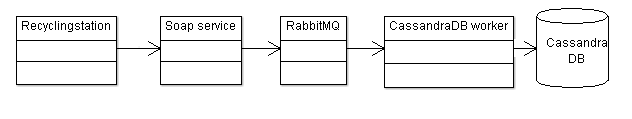
\includegraphics[scale=1]{ClassDiagram.png}

This design is built in such way that it can be scaled and later be replaced or work in conjunction with something written a completely different programming language. This is why there is a queue in between the soapservice and the database worker.

\section{Interfaces}
\subsection{soap}
Because of this interfaces or kept generic or text based (encoded in UTF-8). To deliver something to the soap interface you can either deliver the whole string at once via the addTransactiontext operation of course there is a specific format that should be followed. The format is: "<userID:UUID>, <locationID:UUID> , <timestamp:long> , <paper:int>, <plastic:int>, <glas:int>, <metal:int>". It can also be send in separate parts. The setup is similar but all the parts are separate in the soap message.
\subsection{RabbitMQ}
The RabbitMQ listener expects that all incoming data is a single string encoded in UTF-8. It's expects the data in the format as the string interface of soap.











\end{document}